\section{Application development}

\begin{frame}
\frametitle{Real-time application development}
	\begin{itemize}
		\item A few best-practices should be followed when developing a real-time application
		\item Some POSIX APIs weren't designed with RT behaviour in mind
		\item Some syscalls and memory-access patterns will lead to kernel-side latencies
		\item Following the good practises is important
		\item But benchmarking the application is also crucial
	\end{itemize}
\end{frame}

\begin{frame}
	\frametitle{Initialization}
	\begin{itemize}
		\item Usually, the initialization section of the application doesn't need to be RT
		\item This init section will configure various settings:
			\begin{itemize}
				\item Allocate and lock the memory
				\item Start the threads and configure them
				\item Initialize the locks
				\item Configure the scheduling parameters (priority, deadlines)
				\item Configure the CPU affinity
			\end{itemize}

	\end{itemize}
\end{frame}

%%%%%%%%%
\begin{frame}
  \frametitle{Development and compilation}
  \begin{itemize}
  \item No special library is needed, the POSIX real-time API is part
    of the standard C library
  \item The glibc C library is recommended, as support
    for some real-time features is not mature in other C libraries
    \begin{itemize}
    \item Priority inheritance mutexes or NPTL on some architectures,
      for example
    \end{itemize}
  \item Compile a program
    \begin{itemize}
    \item \code{ARCH-linux-gcc -o myprog myprog.c -lrt}
    \end{itemize}
  \item To get the documentation of the POSIX API
    \begin{itemize}
    \item Install the \code{manpages-posix-dev} package
    \item Run \code{man function-name}
    \end{itemize}
  \end{itemize}
\end{frame}

\begin{frame}
  \frametitle{Process, thread?}
  \begin{itemize}
  \item Confusion about the terms {\em process}, {\em thread} and {\em task}
  \item In UNIX, a process is created using \code{fork()} and is composed of
    \begin{itemize}
    \item An address space, which contains the program code, data, stack, shared
      libraries, etc.
    \item One thread, that starts executing the \code{main()} function.
    \item Upon creation, a process contains one thread
    \end{itemize}
  \item Additional threads can be created inside an existing process, using
    \code{pthread_create()}
    \begin{itemize}
    \item They run in the same address space as the initial thread of
      the process
    \item They start executing a function passed as argument to
      \code{pthread_create()}
    \end{itemize}
  \end{itemize}
\end{frame}

\begin{frame}
  \frametitle{Process, thread: kernel point of view}
  \begin{itemize}
  \item The kernel represents each thread running in the system by
    a \kstruct{task_struct} structure.
  \item From a scheduling point of view, it makes no difference
    between the initial thread of a process and all additional threads
    created dynamically using \code{pthread_create()}
  \end{itemize}
  \begin{center}
    \includegraphics[width=0.8\textwidth]{slides/realtime-linux-application-development/thread-vs-process.pdf}
  \end{center}
\end{frame}

\begin{frame}[fragile]
  \frametitle{Creating threads}
  \begin{itemize}
  \item Linux supports the POSIX thread API
  \item To create a new thread
    \begin{block}{}
\small
\begin{verbatim}
pthread_create(pthread_t *thread, pthread_attr_t *attr,
               void *(*routine)(void*), void *arg);
\end{verbatim}
\normalsize
    \end{block}
  \item The new thread will run in the same address space, but will be
    scheduled independently
  \item Exiting from a thread
    \begin{block}{}
\small
\begin{verbatim}
pthread_exit(void *value_ptr);
\end{verbatim}
\normalsize
    \end{block}
  \item Waiting for the termination of a thread
    \begin{block}{}
\small
\begin{verbatim}
pthread_join(pthread_t *thread, void **value_ptr);
\end{verbatim}
\normalsize
    \end{block}
  \end{itemize}
\end{frame}

\begin{frame}[fragile]
  \frametitle{Using scheduling classes (1)}
  \begin{itemize}
  \item An existing program can be started in a specific scheduling
    class with a specific priority using the \code{chrt} command line tool
    \begin{itemize}
    \item Example: \code{chrt -f 99 ./myprog} \\
        \code{-f}: \ksym{SCHED_FIFO}\\
	\code{-r}: \ksym{SCHED_RR}\\
	\code{-d}: \ksym{SCHED_DEADLINE}
    \end{itemize}
  \item The \code{sched_setscheduler()} API can be used to change the scheduling class
    and priority of a threads
    \begin{block}{}
\begin{verbatim}
int sched_setscheduler(pid_t pid, int policy,
                const struct sched_param *param);
\end{verbatim}
    \end{block}{}
    \begin{itemize}
    \item \code{policy} can be \code{SCHED_OTHER}, \ksym{SCHED_FIFO},
      \ksym{SCHED_RR}, \ksym{SCHED_DEADLINE}, etc. (others exist).
    \item \code{param} is a structure containing the priority
    \end{itemize}
  \end{itemize}
\end{frame}

\begin{frame}[fragile]
  \frametitle{Using scheduling classes (2)}
  \begin{itemize}
  \item The priority can be set on a per-thread basis when a thread is
    created
    \begin{block}{}
\footnotesize
\begin{verbatim}
struct sched_param parm;
pthread_attr_t attr;

pthread_attr_init(&attr);
pthread_attr_setinheritsched(&attr, PTHREAD_EXPLICIT_SCHED);
pthread_attr_setschedpolicy(&attr, SCHED_FIFO);
parm.sched_priority = 42;
pthread_attr_setschedparam(&attr, &parm);
\end{verbatim}
\normalsize
    \end{block}
  \item Then the thread can be created using \code{pthread_create()},
    passing the \code{attr} structure.
  \item Several other attributes can be defined this way: stack size,
    etc.
  \end{itemize}
\end{frame}


%%%%%%%%%

\begin{frame}
	\frametitle{Memory layout and allocation}
	\begin{columns}
		\column{0.3\textwidth}
    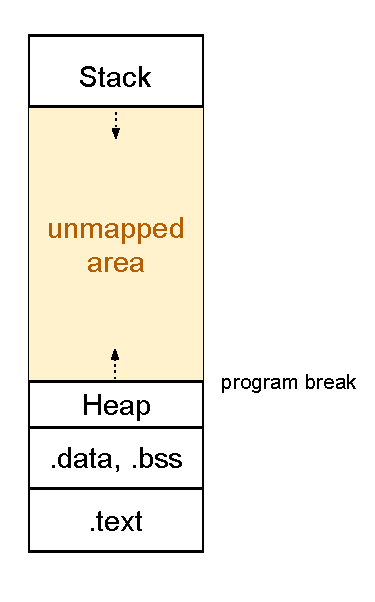
\includegraphics[width=\textwidth]{slides/realtime-linux-application-development/process_memory.pdf}
		\column{0.7\textwidth}
			\begin{itemize}
				\item The \textbf{stack} grows down from high addresses
				\item The \textbf{heap} is used for dynamic allocations, grows up to the \textbf{program break}
				\item \code{mmap()} can also be used to allocate memory in-between
				\item \code{malloc} uses both \code{brk} and \code{mmap}
				\item Allocated memory needs to be \textbf{mapped} to physical memory
				\item Mapping is done per \textbf{page}, usually 4 Kilobytes
				\item It is created when the page is \textbf{first accessed} through a \textbf{page fault}
				\item Each page fault will raise an exception, preempt the process and introduce latency
			\end{itemize}
	\end{columns}
\end{frame}

\begin{frame}[fragile]
	\frametitle{Pre-faulting the stack}
	\begin{columns}
		\begin{column}{0.35\textwidth}
    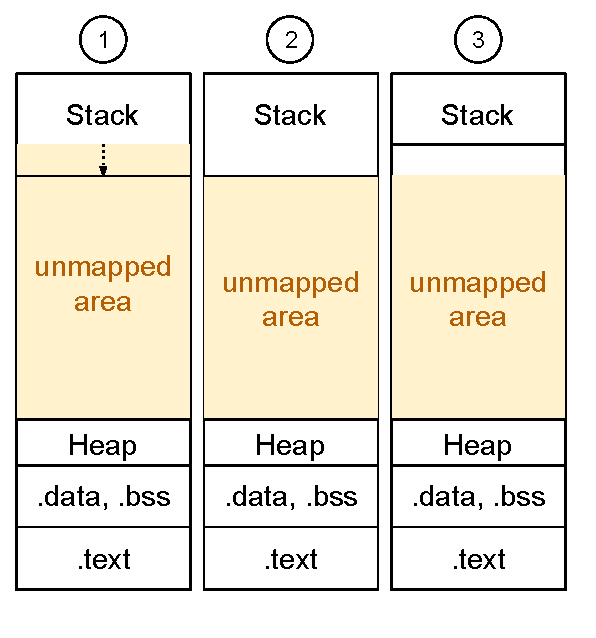
\includegraphics[width=\textwidth]{slides/realtime-linux-application-development/prefault_stack.pdf}
		\end{column}
		\begin{column}{0.65\textwidth}
			\begin{enumerate}
				\item Allocate huge buffers on the stack in a sub-function
				\item Access (read or write) the whole buffer
				\item return from the sub-function
			\end{enumerate}
			\begin{block}{stack prefault}
			\fontsize{8}{7}\selectfont
				\begin{minted}{c}
#define BUFSZ (1024 * 1024 * 8)
static void stack_prefault() {
        char buff[BUFSZ];
        long page_sz;
        int i;

        page_sz = sysconf(_SC_PAGESIZE);

        for (i = 0; i < BUFSZ; i += page_sz)
                buf[i] = 0;
}
				\end{minted}
			\end{block}
		Each thread's stack must be pre-faulted
		\end{column}
	\end{columns}

\end{frame}

\begin{frame}
	\frametitle{Pre-faulting the heap}
	\begin{columns}
		\column{0.25\textwidth}
    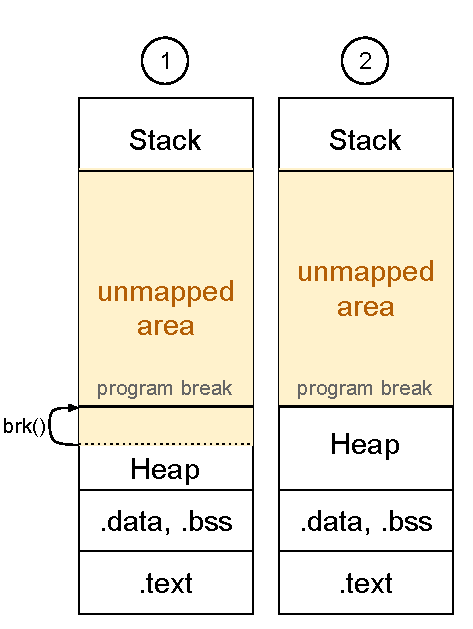
\includegraphics[width=\textwidth]{slides/realtime-linux-application-development/prefault_heap.pdf}
		\column{0.75\textwidth}
			\begin{itemize}
				\item The \textbf{program break} defines the size of the \code{.data} segment
				\item \code{malloc} uses the \code{.data} segment as a pool for small buffers
				\item Prevent the program break from shrinking
					\begin{itemize}
						\item \code{mallopt(M_TRIM_THRESHOLD, -1);}
					\end{itemize}
				\item Prevent \code{malloc} from using \code{mmap}
					\begin{itemize}
						\item By default, \code{malloc} uses \code{mmap} for large buffers
						\item Once free'd, mmap'd pages won't be re-used
						\item \code{mallopt(M_MMAP_MAX, 0);}
					\end{itemize}
				\item allocate a huge buffer to move the program break
				\item Access the whole buffer
				\item \code{free()} the buffer
				\item Subsequent calls to \code{malloc} will re-use pre-faulted memory
				\item For multi-threaded applications, pre-fault each \textbf{arena}
					\begin{itemize}
						\item see \code{M_ARENA_TEST} and \code{M_ARENA_MAX} \code{mallopt} options
					\end{itemize}
			\end{itemize}
	\end{columns}

\end{frame}

\begin{frame}
	\frametitle{Memory management}
	\begin{itemize}
		\item Call \code{mlockall(MCL_CURRENT | MCL_FUTURE)} at init to lock all memory regions
		\item This prevents mapping from being removed
		\item Beware of \code{fork()}, since the child will copy-on-write pages
		\item \code{malloc}'s implementation is libC specific
		\item \textbf{glibc} implements all the necessary options
		\item \textbf{musl} doesn't implement \code{mallopt} and may use \code{mmap}
		\item \textbf{ftrace} can be used to trace pagefaults :
			\begin{itemize}
				\item \code{trace-cmd record -e page_fault* <cmd>}
			\end{itemize}
	\end{itemize}
\end{frame}

\begin{frame}
	\frametitle{Locking}
	\begin{itemize}
		\item When creating multi-threaded applications, use \code{pthread_mutex_t}
		\item Avoid using semaphores, which don't have an owner
		\item These are POSIX mutexes, which have a notion of \textbf{ownership}
		\item Ownership allows to handle \textbf{Priority Inheritance} (PI)
		\item PI needs to be explicitely enabled: \code{pthread_mutexattr_setprotocol(&mattr, PTHREAD_PRIO_INHERIT);}
	\end{itemize}
\end{frame}

\begin{frame}
	\frametitle{Synchronizing and signaling}
	\begin{itemize}
		\item Application might need to wait or react to external events
		\item Inter-thread signaling should be done with \code{pthread_cond_wait()}
		\item Conditions can be attached to mutexes
		\item Avoid using UNIX Signals
	\end{itemize}
\end{frame}

\begin{frame}
	\frametitle{timekeeping}
	\begin{itemize}
		\item Usually, real-time applications will need timing information
		\item This can be done by using \code{clock_gettime(clk_id, &ts)}
		\item Although counter-intuitive, don't use the \code{CLOCK_REALTIME} clock id
		\item \code{CLOCK_REALTIME} gives the current time, which can be adjusted and is non-consistent
		\item Instead, use \code{CLOCK_MONOTONIC} which is never adjusted and strictly increasing
	\end{itemize}
\end{frame}
